\chapter{KURIKULUM}
\label{kurikulum}
Pojem kurikulum je odvozen z latinského slova \textit{currere} tedy běžet.  Slovo curriculum má významy jako \textit{\uv{běh, závodiště či závodní vozík}}. Může to tedy znamenat \textit{\uv{pohyb po určité trase, směrem k určitému cíli}} \citep[s.~24]{Opravilova}. Nejčastěji je dnes toto slovo používané jako curriculum vitae neboli životopis, běh života. V češtině se používá jeho přepis kurikulum.

Ve spojení s pedagogikou se tento pojem začíná užívat v zahraničí v 60. letech 20. století. Dá se chápat jako plánovaná a~nasměrovaná trasa, na níž dítě získává zkušenosti dle svých schopností a~zájmů. V České republice se tento pojem užívá až koncem 80. let. Existuje mnoho jeho definic a~významů podle různých pedagogických koncepcí a~názorů samostatných autorů.

K rozšíření pojmu kurikulum u~nás významně přispěla Eliška Walterová. Díky ní se dostal do české odborné pedagogické terminologie. Pro tuto práci se hodí dva významy podle \citet[s.~15]{Walterova}:

\uv{\textit{\textbf{Vzdělávací program, projekt, plán:} 
		zahrnuje škálu od programu jednotlivého kurzu nebo vyučovacího předmětu až po komplexní program vzdělávací instituce, tj. plán všech aktivit ve škole;}

\textit{\textbf{Průběh studia a~jeho obsah:}
		charakteristika vzdělávací dráhy a~obsah zkušeností, kterou žák získává v době studia.}}

\citet[s.~237]{Prucha} definuje kurikulum jako \uv{\textit{obsah vzdělávání, který zahrnuje veškeré zkušenosti, které žáci získávají ve škole a~v činnostech ke škole se vztahujících, zejména jejich plánování, zprostředkovávání a~hodnocení.}}

Dle terminologie se dělí kurikulum na \textbf{formální}, \textbf{neformální} a~\textbf{skryté}. Tato práce se zabývá kurikulem formálním. Formální kurikulum je komplexní projekt cílů, obsahu, prostředků a~organizace vzdělávání, realizace projektovaného kurikula, způsoby kontroly a hodnocení výsledků.

Kurikulární dokumenty jsou v~obou srovnávaných zemích pojímány odlišně. Ve Francii je kurikulum předškolní výchovy zahrnuto v~jednom dokumentu s~kurikulem školy základní (vysvětleno v~kapitole \ref{frkurikulum}). V~České republice je naopak předškolnímu vzdělávání věnován samostatný dokument, který se zabývá širokým spektrem otázek ohledně vzdělávání nejmenších dětí. Pro tuto práci byly vybrány srovnatelné parametry, které se nacházejí v obou dokumentech. Za účelem jejich porovnání je v této práci brán pojem kurikulum jakožto vzdělávací program či obsah vzdělávání a~pozornost je věnována \textbf{vzdělávacím oblastem předškolního vzdělávání} a~\textbf{kompetencím}, které by děti měly zvládat na konci mateřské školy. Pro jasnější představu o~dokumentech obou zemí je na začátku každé kapitoly zmíněno i~legislativní pojetí kurikula, jeho dostupnost a~stručný přehled, jak celý dokument vypadá. 

	\section{Francouzské kurikulum}
	\label{frkurikulum}

		Mateřská škola ve Francii je součástí preprimárního vzdělávání, odpovídající úrovni ISCED~0. Jak bylo uvedeno v~kapitole \ref{msvefr}, vzdělávání dětí předškolního a~školního věku je řazeno do tří cyklů. Na půdě školy mateřské se odehrávají první dva cykly. Cílem preprimárního vzdělávání je připravit dítě na vstup do povinného vzdělávání na základní škole a~zaručit plynulý přechod podle individiuálních schopností každého dítěte. Francouzské kurikulum předškolního vzdělávání je tedy součástí stejného dokumentu jako kurikulum školy základní. Legislativně je zakotveno ve školském zákoně (Code de l´éducation) č. 2003-339, který vešel v platnost 14. června 2003.
	
		Francouzské kurikulum je veřejně dostupný dokument, který je vydáván v~podobě bulletinu Ministerstvem školství a~výzkumu \citep{buletin}. Vychází též v knižní verzi od CNDP (Centre National de Documentation Pédagogique)\citep{CNDP}.

		Část dokumentu týkající se předškolního vzdělávání, která je v~této práci předložena, nebyla ještě z~francouzského jazyka přeložena a~otvírá novou oblast pro českého čtenáře. Níže je prezentován vlastní autorčin překlad vzdělávacích oblastí, nejedná se tedy o~překlad oficiální. 

		Francouzský kurikulární dokument obsahuje následujících 11 kapitol: 

	\begin{enumerate}[1]
		\setlength\itemsep{-2mm}
		\item Dopis od bývalého ministra školství Xaviera Darcose k novým programům primárního vzdělávání \textit{(Lettre de Xavier Darcos sur le noueaux programmes pour l´école primaire.)}
		\item Hodinová dotace v mateřské a~základní škole \textit{(Horaires des écoles maternelles et élémentaires)}
		\item Program primárního vzdělávání \textit({Programmes d´enseignement  de l´école primaire)}
		\item Preambule \textit{(Préambule)}
		\item Prezentace \textit{(Présentation)}
		\item Program mateřské školy: nižší stupeň, střední stupeň, vyšší stupeň \textit{(Programme de l´école maternelle:petite section, moyenne section, grande section)}
		\item Cyklus základního vzdělávání - Program CP a~CE1 \textit{(Cycle des apprentissages fondamentaux – Pogramme du CP et du CE1)}
		\item Cyklus prohlubování vzdělání – Program CE2, 1 a~CM2 \textit{(Cycle des approfondissements – Programme du CE2, du CM1 et du CM2)}
		\item Kritéria organizace progresivity vzdělávání v mateřské škole \textit{(Repères pour organiser la progressivité des apprentissages à l´école maternelle)}
		\item Cyklus základního vzdělávání – Postup pro CP a~CE1 \textit{(Cycle des apprentissage fondamentaux – Progression pour le cours préparatoire et le cours élémentaire)}
		\item Cyklus prohlubování – Postup pro CE2, CM1 a~CM2 \textit{(Cycle des approfondissements pour le cours élémentaire dèuxieme année et le cours moyen)}
	\end{enumerate}


	Mateřskou školou a~programem vzdělávání se v~dokumentu zabývá šestá kapitola.

	Program pro mateřské školy je rozdělen do 6ti hlavních vzdělávacích oblastí, které jsou dále členěny do několika oblastí dílčích.
	
	\begin{enumerate}[1]
		\setlength\itemsep{-2mm}
		\item Osvojit si řeč 
		\item Objevovat písmo 
		\item Stát se žákem 
		\item Jednat a~vyjadřovat se vlastním tělem 
		\item Objevovat svět
		\item Vnímat, cítit, představovat si, tvořit
	\end{enumerate}

Na konci každé vzdělávací oblasti jsou uvedeny znalosti a~dovednosti, které by děti měly ovládat na konci mateřské školy. Jedná se o~základy kompetencí, ke kterým je dítě vedeno, ale nejsou překážkou v~postupu do dalšího ročníku/cyklu.

		\subsection{Osvojit si řeč (S'approprier le langage)}
			Mluvený jazyk je v mateřské škole základním pilířem učení. Vyjadřování a~pochopení se dítě učí skrze jazyk. Učí se být pozorný ke zprávě, která je mu sdělena, pochopit ji a odpovědět na ni. V rámci komunikace s učitelem, kamarády a~při společných i~specificky zaměřených aktivitách, se každodenně učí novým slovům. Postupně si osvojuje syntaxi francouzského jazyka. Společné aktivity obohacují slovní zásobu a~způsoby užití jazyka (dotazování se, vyprávění, vysvětlování, přemýšlení).

			\paragraph{Komunikovat, vyjadřovat se (Échanger, s´exprimer)}

			Nejdříve se děti učí komunikovat prostřednictvím dospělého v situacích, které se ho přímo týkají: jejich vlastní potřeby, objevy, otázky; naslouchá a~odpovídá na žádosti. S jistotou pojmenovává objekty okolo sebe. Účastní se komunikace ve skupině, čeká, až na něj přijde řada a~možnost vyjádřit se a~respektuje dané téma. Dokáže nazpaměť převyprávět naučené říkanky a~písně. Pozvolna rozšiřuje časovou osu, mluví o~tom, co se bude dít, co zažilo, dokáže vymýšlet příběhy a~převyprávět základní fakta problému. Postupně získává potřebné základy jazyka k vyjádření se: popis osob a~vztahů mezi nimi, užití správného časování sloves a~jak vhodným způsobem popsat dění v příběhu.

			\paragraph{Porozumět (Comprendre)}
			Více než vyjadřování je základní kapacitou dítěte porozumění, na které je kladen v tomto věku velký důraz.
			Děti se učí rozlišovat otázku, slib, příkaz, odmítnutí, vysvětlení, vyprávění. Rozumí příkazům vyučujícího a~všem termínům, které k tomu patří. Jsou vedené k pochopení kamaráda či dospělého, který hovoří o~věcech pro dítě neznámých. Opakováním příběhů a pohádek, jak klasické tak moderní literatury, které jsou přiměřené věku dětí, je dětem umožněno porozumět složitějším a~delším vyprávěním, která dokážou též převyprávět. 

			\paragraph{Zdokonalovat se ve francouzském jazyce (Progresser vers la maîtrise de la langue française)}
			Užíváním jazyka a~posloucháním čtených textů se dítě učí pravidlům větné skladby a pořadí slov ve francouzské větě. Na konci mateřské školy dítě ovládá všechny slovní druhy, tvoří celé věty i~krátká vyprávění a~vysvětlení. Každodenní čtení a~vyprávění příběhů učitelem, která obsahují nová slova, nestačí k jejich zapamatování. Nabytí slovní zásoby vyžaduje specifický přístup, pravidelné aktivity na klasifikaci a~memorizování slov, opakované používání slov již naučených a~vysvětlování neznámých termínů v jejich kontextu. Učitel dohlíží, aby se každý týden děti naučily nová slova obohacující slovní zásobu. Děti se učí nejen slovíčka, která jim pomáhají k pochopení mluveného textu, ale také slova k efektivní komunikaci ve škole a~k~co nejpřesnějšímu vyjádření vlastních myšlenek. Vyučující věnuje každému dítěti dostatek pozornosti, pomáhá mu se správnými slovy a~podporuje ho. Přeformuluje pokus dítěte, aby slyšelo, jak zní správný model. Aby se děti mohly zdokonalovat v mluveném projevu, je jim vyučující příkladem správnosti vět a~přesné slovní zásoby.

			\paragraph{Znalosti a~dovednosti, které by děti měly ovládat na konci MŠ}
			\begin{itemize}
				\setlength\itemsep{-2mm}
				\item[-] porozumět zprávě a~reagovat nebo odpovědět na ni vhodným způsobem
				\item[-] s jistotou popsat objekt, osobu nebo událost z běžného života
				\item[-] srozumitelně vyjádřit otázku nebo popis
				\item[-] srozumitelně vyprávět pro posluchače neznámý příběh nebo příběh vymyšlený 
				\item[-] iniciativně se ptát na otázky a~vyjadřovat svůj vlastní názor
			\end{itemize}


		\subsection{Objevovat písmo (Découvrir l'écrit)}
			Mateřská škola připravuje děti na základní vzdělávání. Činnosti spojené s mluveným projevem, navyšování slovní zásoby, písemná tvorba a~četné poslechy vyprávěného a~čteného textu učí žáky dovednostem čtení a~psaní. Tři klíčové aktivity (cvičení na zvukovou stránku slov \uv{fonémy}, na základy abecedy a~grafomotoriku) v mateřské škole významně podporují systematickou přípravu na čtení a~psaní, která začíná v přípravném vzdělávání (CP-cours préparatoir).

			\paragraph*{I Seznámit se s psaním (Se familiariser avec l´écrit)}
				\subparagraph{Objevování psaných podkladů (Découvrir les supports de l´écrit)}
					Děti objevují užívání písemného projevu ve společnosti srovnáváním psaných podkladů, ve škole i~mimo ni (plakáty, knihy, noviny, časopisy atp.). Učí se ho přesně popsat a pochopit jeho funkci. Objevují a~používají knihy, učí se orientovat na stránce i~na přebalech knih. 
				\subparagraph{Objevování psaného jazyka (Découvrir la langue écrite)}
					Díky čteným textům se děti každý den seznamují s psanou francouzštinou. Aby mohly vnímat specifika psaného projevu, jsou vybírány texty jazykově kvalitní z různých literárních žánrů (pohádky, legendy, bajky, básně, říkanky). Po celou dobu mateřské školy jsou děti vedeny k vyprávění a~osvojování si děl z literárního dědictví. Stávají se citlivější ke způsobům, jak vyjádřit méně známé skutečnosti. Jejich zvědavost je stimulována otázkami vyučujícího, který zdůrazňuje nová slova a~slovní obraty, které poté používá i v jiných situacích.  Děti vyprávějí přečtený příběh, sdělují, co pochopily, a~doptávají se na nejasnosti. Jsou povzbuzovány k memorizování vět nebo krátkých úryvků textu. 
				\subparagraph{Základy psaní textu (Contribuer à l´écriture de textes)}
					Děti se účastní činností, jež přirozeně zanechávají stopu toho, co se stalo, bylo pozorováno nebo naučeno. Učí se diktovat text dospělému. Ten jim případnými otázkami pomáhá uvědomit si požadavky formy vyřčeného. Jsou též vedeny ke správnému výběru slov a syntaktické struktuře. Na konci mateřské školy dovedou děti transformovat spontánní mluvený projev na text, který dokáže dospělý zapsat podle diktátu.

				\subparagraph{Znalosti a~dovednosti, které by děti měly ovládat na konci MŠ} 
				\begin{itemize}
					\setlength\itemsep{-2mm}
					\item[-] rozlišovat zvuky
					\item[-] poznat slabiky vyřčeného slova, poznat stejnou slabiku v různých slovech
					\item[-] rozeznat a~napsat většinu písmen abecedy
					\item[-] spojit hlásku s písmenem
					\item[-] pod vedením učitele napsat krátká jednoduchá slova z hlásek a~písmen, které děti již znají 	
					\item[-] napsat své jméno
				\end{itemize}


			\paragraph*{II Připravit se na čtení a~psaní (Se préparer à apprendre à lire et~à~écrire)}
				\subparagraph{Rozeznávání zvuku slov (Distinguer les sons de la parole)}
					Děti velmi brzy objevují radost ze hry se slovy a~zvukomalebností jazyka. Nejdříve slabiky pokřikují, později si s nimi hrají (vynechávají slabiky, kombinují několik slabik dohromady v různém pořadí). Dokážou rozeznat stejné slabiky v jiných slovech a~určit jejich pozici ve slově (na začátku, uprostřed, na konci).
					Postupně rozlišují zvuky hlásek a~učí se operovat s nimi a~s~dalšími jazykovými komponenty. Vyučující je pozorný k pokroku při osvojování si abstraktních hlasových aktivit.
				\subparagraph{Základy abecedy (Aborder le principe alphabétique)}
					Děti se seznamují se základy rozdílnosti mezi mluveným a~psaným projevem francouzského jazyka. Pozorováním známých věcí (datum, název příběhu nebo pohádky) nebo krátkých vět děti porozumí posloupnosti slov a~faktu, že každé napsané slovo odpovídá slovu mluvenému. 
					Objevují, že každé slovo, které řeknou nebo které slyší, je složeno ze slabik a~dávají si do spojitosti písmena a~hlásky. Rozlišování hlásek je čím dál tím přesnější. Postupně se učí názvy všech písmen abecedy, která umí rozpoznat napsané tiskacím i~psaným písmem, i~přesto, že klasické pořadí písmen v abecedě jim ještě zůstává neznámé. U~některých písmen si k~jejich názvu asociují zvuk hlásky (pozn. autorky – názvy písmen abecedy ve francouzském jazyce jsou odlišné od hlásek daných písmen ve slově). Tímto si osvojují principy abecedy.
				\subparagraph{Základy grafomotoriky (Apprendre les gestes de l´écriture)} 
					Každý den děti pozorují a~reprodukují grafické motivy. Tím se učí nejefektivnějším gestům (pohybům). Vstup do světa psaní záleží na rozvinuté grafomotorice (spojování jednoduchých linií, vln apod.), ale vyžaduje i~zvláštní dovednosti vnímat charakteristiky písmen. 
					Děti na vyšším stupni (Grande section), které na to již mají kapacity, je předkládáno i písmo psané. Jde o~řízenou aktivitu pod dohledem vyučujícího. První zvyky, které si dítě osvojí, mají vliv na pozdější kvalitu zápisu a~uvolněnost ruky při psaní. 
					
					\subparagraph{Znalosti a~dovednosti, které by děti měly ovládat na konci MŠ}
					\begin{itemize}
						\setlength\itemsep{-2mm}
						\item[-] rozpoznat hlásky
						\item[-] rozlišovat slabiky vyřčených slov, poznat stejné slabiky v různých slovech
						\item[-] z krátkého výroku pospojovat mluvená slova s napsanými
						\item[-] rozpoznat a~napsat většinu písmen abecedy
						\item[-] pojit hlásku s písmenem
						\item[-] pod vedením vyučujícího kopírovat psaným písmem krátká a~jednoduchá slova, která dítě již zná
						\item[-] napsat psacím písmem své jméno
					\end{itemize}


		\subsection{Stát se žákem (Devenir élève)}
			Cílem je dítě naučit, co ho odlišuje od ostatních a~vnímat sám sebe jako osobnost a~naučit ho žít v organizované společnosti s pravidly. Chápat, co je to škola a~jaké je v ní jeho místo. Stát se žákem je postupný proces, který od vyučujícího vyžaduje jak flexibilitu, tak důslednost.
			\paragraph{Život ve společnosti: jak se naučit pravidla společnosti a~základy slušného chování (Vivre ensemble: apprendre les règles de civilité et les principes d´un comportement coforme à la morale)}
				Děti objevují bohatství i~nátlak skupiny, do které jsou začleňovány. Pociťují radost z přijetí, že jsou poznány a~postupně přijímají i~ostatní kamarády. Kolektiv, ve kterém se děti v mateřské škole nacházejí, tvoří vhodné prostředí, kde se učí vést dialog mezi sebou, s dospělými a~učí se, kdy na ně přijde řada. Je to výborná příležitost k nácviku pravidel slušného chování, jako je pozdravit na začátku a~na konci dne, odpovědět na otázku, poděkovat osobě, která nám pomohla a~nepřerušovat ostatní. Zvláštní důraz je kladen na morální základy pravidel chování, jako je respektování ostatních osob a~dobro bližních, povinnost přizpůsobit se pravidlům daných dospělými i~respektovat, že mluví druhé dítě. 

			\paragraph{Spolupráce a~samostatnost (Coopérer et devenir autonome)}
				Účast ve hrách, kruzích či vytvořených skupinkách, kde mají děti recitovat říkanku nebo poslouchat příběh, účast na realizaci společných projektů apod., jsou aktivity, díky kterým děti přicházejí na chuť společným činnostem a~učí se spolupracovat. Zajímají se o~ostatní a spolupracují s nimi. Přebírají zodpovědnost ve třídě a~jsou iniciativní. Angažují se v projektech nebo činnostech s důrazem na své vlastní zdroje. Zakoušejí samostatnost, úsilí a~vytrvalost. Učí se chápat, co to je škola.
				Děti se mají postupně naučit, jaká jsou pravidla školní komunity, specifika školy, co se ve škole dělá, co se od nich očekává a~co a~proč se ve škole učí. Rozlišují rozdílné role rodičů a~učitelů. 
				Postupně přijímají rytmus společných činností a~dokážou odlišit uspokojení z jejich vlastních zájmů. Chápou hodnotu společných pravidel. Učí se, jak klást otázky a jak vyjednávat, aby dosáhly zadaného. Rozvíjejí si souvislosti mezi materiálními činnostmi a~tím, co se danou aktivitou učí. Získávají objektivní kritéria pro evaluaci vlastních úspěchů. Na konci mateřské školy umí poznat vlastní chyby i~chyby kamarádů. Postupně se učí delšímu soustředění. Objevují spojení mezi tím, co se učí a~věcmi v běžném životě.
			\paragraph{Znalosti a~dovednosti, které by děti měly ovládat na konci MŠ}
			\begin{itemize}
				\setlength\itemsep{-2mm}
				\item[-] respektovat ostatní a~respektovat pravidla společného života
				\item[-] poslouchat, pomáhat, spolupracovat, žádat o~pomoc
				\item[-] důvěřovat sám sobě, kontrolovat vlastní emoce
				\item[-] identifikovat dospělé a~jejich role
				\item[-] být samostatný v jednoduchých úkonech a~hrát roli ve školních činnostech
				\item[-] říct, co se naučilo
				\end{itemize}

		\subsection{Jednat a~vyjadřovat se vlastním tělem (Agir et s'exprimer avec son corps)}

			Fyzická aktivita a~zkušenosti s vlastním tělem přispívají k rozvoji motoriky, smyslů, citů a intelektu dítěte. Jsou příležitostí objevovat, vyjádřit se, jednat ve známém prostředí, později i~v~prostředí méně známém a~dovolují orientovat se v prostoru. Dítě objevuje možnosti svého těla. V bezpečí se učí reagovat a~přijímat možná rizika a~využití adekvátního množství energie pro danou činnost. Vyjadřuje, co cítí, dokáže popsat činnosti a~objekty, s kterými pracuje a~používá je. Vyjadřuje, co má chuť dělat. Vyučující zaručuje  pestrou nabídku činností, zvyšování jejich náročnosti a~dostatek možností ke sebezdokonalování. Také jim pomáhá vytvářet důvěru sám v sebe a~v nově nabytých dovednostech. 
			\textbf{Skrze fyzickou aktivitu řízenou nebo volnou} v různých prostředích rozvíjejí děti své motorické dovednosti, rovnováhu, manipulaci, házení a~chytání. Hry s míčem, hry s protivníkem, hry s pravidly doplňují tyto aktivity. Děti řídí dané aktivity i~jejich návaznost. Osvojují si motorické dovednosti, kdy je správně používat a~jejich správné provedení. 
			\textbf{Skrze činnosti s pravidly} rozvíjejí dovednosti adaptace a~spolupráce. Díky nim chápou a přijímají pozitiva a~negativa činností v kolektivu. 
			\textbf{Umělecké činnosti} jako kruh, tanec a~pantomima pomáhají k vyjádřování se gesty a~k~rozvoji představivosti.
			Pomocí rozličných činností nabývají děti \textbf{obraz vlastního těla}. Rozlišují před, za, nahoře, dole, vpravo, vlevo, blízko a~daleko. Zvládají překážkové dráhy a~dokážou popsat své pohyby a~jejich provedení.
				\paragraph{Znalosti a~dovednosti, které by děti měly ovládat na konci MŠ}

				\begin{itemize}
					\setlength\itemsep{-2mm}
					\item[-] přizpůsobit své pohyby v různých prostředích a~omezeních
					\item[-] individuálně či společně pracovat nebo být proti
					\item[-] vyjádřit se hudebním rytmem, nástrojem, vyjádřit své pocity a~emoce gesty a~pohyby
					\item[-] orientovat se a~pohybovat se v prostoru
					\item[-] popsat a~vytvořit jednoduchou dráhu
				\end{itemize}

		\subsection{Objevovat svět (Découvrir le monde)}
			V mateřské škole dítě objevuje svět okolo sebe. Učí se prostorovým a~časovým omezením a jak se jim přizpůsobovat. Pozoruje, klade otázky a~dělá pokroky v účelnosti dotazování. Učí se přijímat jiný pohled na věc než svůj vlastní.  Konfrontace a~logické myšlenky mu dodávají chuť uvažovat nad věcmi. Naučí se počítat, třídit, uspořádávat a~popsat věci jak jazykem, tak různými formami vyjadřování (obrázky, náčrty). Začíná chápat rozdíly mezi živými a~neživými objekty.

			\paragraph{Objevování objektů (Découvrir les objets)}
				Děti objevují běžné technické předměty (baterka, telefon, počítač atd.), chápou jejich využití a~funkce, k čemu slouží a~jak je používat. Naučí se i~znaky nebezpečných předmětů.
				Vyrábějí předměty s~využitím různých materiálů a~vybírají si vhodné nástroje a~techniky (stříhání, lepení, ohýbání, skládání, připíchnutí, složení a~rozložení atd.).
			\paragraph{Objevování materiálu (Découvrir la matière)}
				Znalosti o~charakteristických vlastnostech materiálů získávají děti díky činnostem, jako je stříhání, modelování, spojování běžných materiálů (dřevo, půda, papír, karton, voda, atd.).
				Uvědomují si i~méně viditelnou realitu jako např. vítr, a~začínají vnímat změny skupenství vody. 
			\paragraph{Objevování živého (Découvrir le vivant)} 
				Děti objevují různé projevy živé přírody. Chov dobytka a~hospodářství jsou významným prostředkem k objevování cyklu života od narození přes růst, reprodukci, po stárnutí až smrt.
				Objevují části těla a~pět smyslů, jejich charakteristiku a~funkci. Zajímají se o~hygienu, zdraví a~zejména o~stravu. Učí se základním pravidlům hygieny těla. 
				Jsou vnímavé k problémům životního prostředí a~učí se respektovat život. 
			\paragraph{Objevování formy a~rozměrů (Découvrir les formes et les grandeurs)}
				Manipulací s různými předměty děti odhalují nejdříve jednoduché vlastnosti (malý/velký; těžký/lehký) a~poté dokážou rozlišovat základní kritéria, srovnávat a~třídit podle tvaru, velikosti, množství a~obsahu.
			\paragraph{Přibližování se veličinám a~číslům (Découvrir les quantités et les nombres)}
				Mateřská škola je klíčovým obdobím k získání povědomí o~posloupnosti čísel a~jejich využití v určování množství. Děti objevují a~učí se chápat funkce čísel, zvláště jako prostředek k~vyjádření množství a~označení pořadí objektů v řadě.
				Činnosti jako rozdělování, srovnávání a~třídění ovlivňují přístup dětí k vnímání celku. Děti se postupně učí počítat nejméně do třiceti a~základům jednoduchých počtů.
				Čísla jsou používána v situacích, které dávají dětem smysl a~jsou praktickým prostředkem k dosažení cíle: hry, činnosti ve třídě, zadané úkoly na srovnávání, spojování, řazení a rozdělování. Velikost celku a~možnost reagovat na předměty jsou důležité proměnné, které vyučující přizpůsobuje kapacitám každého dítěte. 
				Konec mateřské školy je časem prvních kroků do světa počtů. 
				Tím je psaní číslic v konkrétních situacích (např. kalendář) nebo při hrách (přemísťování se po značkách s číslicemi). Děti si vytvářejí první spojení mezi ústním označením a~psaným označením číslic. Jejich výkon zůstává velmi rozdílný, ale je důležité, aby se začali této dovednosti učit. K výuce psaní číslic se přistupuje stejně důkladně jako v případě psaní písmen.
			\paragraph{Orientace v čase (Se repérer dans le temps)}
				Pravidelnou organizací rozvrhu děti pozvolna vnímají časovou posloupnost dnů, týdnů, měsíců. Na konci mateřské školy chápou cykličnost určitých fenoménů (roční období) a znázornění času (týden, měsíc). Toto učení se pojmu je utvrzováno v činnostech i ve známých příbězích. Grafické znázornění napomáhá k~jejich utvrzení (obrázky, kresby).
				V nižším stupni (Petite section) používají děti k orientaci v chronologii a~měření času kalendáře, hodiny a~přesýpací hodiny. V přípravné třídě se tyto limitované znalosti prohlubují. Popisováním příběhů, které se již staly, nebo pozorováním rodinného odkazu, se děti učí blízké minulosti a~s většími obtížemi i~vzdálené budoucnosti.
				Tyto činnosti dávají prostor k učení se přesné slovní zásoby, která je opakovaným používáním, zvláště při rituálech, fixována.
			\paragraph{Orientace v prostoru (Se repérer dans l´espace)}
				Po celou dobu mateřské školy se děti učí pohybovat se po prostorách a~nejbližším okolí školy. Dokážou si najít své místo ve vztahu k věcem a~ostatním osobám a~lokalizovat věci a~osoby v~prostoru, což předpokládá schopnost oprostit se od svého vlastního pohledu na věc. Na konci mateřské školy rozlišují pravou a~levou stranu. Děti zvládnou projít trasu podle značek a~povelů (příkazy a~grafické znázornění).
				Činnosti, při kterých děti musí přecházet z vertikálního plánu do horizontálního, a~naopak, a udržovat relativní postavení předmětů nebo znázorněné prvky, jsou předmětem mimořádné pozornosti. Připravují je na orientaci v grafickém prostoru. Orientace v prostoru na stránce nebo na papíře a~orientace na lince je spojena s dovednostmi čtení a psaní. 
			\paragraph{Znalosti a~dovednosti, které by děti měly ovládat na konci MŠ}
				% HACK
				\vspace{-2mm}
				\begin{itemize}
					\setlength\itemsep{-2mm}
					\item[-] rozeznat, vyjmenovat, popsat, porovnat, uspořádat, třídit materiál a~předměty podle jejich kvalit a~užití
					\item[-] znát projevy života zvířat i~rostlin, spojit je s vyšší funkcí: narození, výživa, pohyb, reprodukce
					\item[-] vyjmenovat hlavní části těla a~jejich funkce, rozlišit pět smyslů a~k čemu slouží
					\item[-] umět a~aktivně užívat pravidla hygieny těla, prostředí, stravování
					\item[-] rozpoznat a~uvědomovat si nebezpečí
					\item[-] orientovat se ve dnech, týdnech, měsících
					\item[-] dokázat určit událost ve vztahu k ostatním událostem
					\item[-] nakreslit kruh, čtverec, trojúhelník
					\item[-] porovnat počet, vyřešit početní úkol
					\item[-] umět nazpaměť, jak jdou číslice do třiceti za sebou 
					\item[-] slovně vyjádřit  množství v~číslicích 
					\item[-] orientovat se v prostoru a~oproti ostatním předmětům
					\item[-] orientovat se na stránce
					\item[-] užívat správná slovní vyjádření při popisu vztahu času a~prostoru
				\end{itemize}

		\subsection{Vnímat, cítit, představovat si, tvořit (Percevoir, sentir, imaginer, créer)}
			Mateřská škola nabízí první setkání s citem pro umění. Vizuální, hmatové, sluchové a hlasové činnosti zvyšují smyslové schopnosti dětí. Pobízí jeho představivost a~obohacují jeho vyjadřovací znalosti a~kapacity. Přispívají k rozvoji pozornosti a~koncentrace. Poslech a~pozorování jsou příležitostmi seznámit dítě s formami uměleckého vyjádření. Poznávají své emoce a~vstupují do uměleckého světa.
			Tyto činnosti souvisejí též s ostatními obory vzdělávání, podporují zvídavost k objevování světa, dovolují dětem vyjadřovat se pohybem, podporují vyjádření vlastních reakcí a~chutí a~dávají možnost výběru v~rámci interakce s ostatními.
			\textbf{Výkresy a~prostorové kompozice (výroba předmětů) jsou oblíbenými prostředky vyjadřování.}
			Děti experimentují s mnoha nástroji, které jim pomáhají tvořit výkresy. Objevují, používají předměty různé povahy a~realizují obrazy. Tvoří předměty využitím malby, lepením papíru, koláží, asambláží, modelováním apod.
			V tomto kontextu vyučující pomáhá dětem vyjádřit to, co vnímají, a~podporuje vlastní zahájení projektů a~jejich realizaci. Přitom je učí používání správných slov. Povzbuzuje děti, aby si založily osobní sbírku předmětů s estetickou a~citovou hodnotou.
			\textbf{Hlas a~sluch} jsou prostředky komunikace, které děti velmi brzo objevují při hře se zvuky, při zpěvu a~při pohybu.
			Repertoár říkanek a~písní vycházející z ústní tradice, do které spadají i~moderní autoři, se každým rokem obohacuje. Děti zpívají pro radost a~hrají si s hlasem, hlukem a~rytmy.
			Strukturované poslechové činnosti bystří pozornost, rozvíjejí citlivost rozlišovat zvuky a zvukovou paměť. Děti poslouchají zvuky pro zábavu, za účelem jejich napodobování, kvůli pohybu a v rámci hry. Učí se rozlišovat barvu, intenzitu, dobu, výšku tónu. Srovnávají, napodobují a~určují jejich znaky. Poslouchají různá hudební díla. Hledají nové možnosti užití hudebních nástrojů. Po částech se učí rytmus a~tempo. 

			\paragraph{Znalosti a~dovednosti, které by děti měly ovládat na konci MŠ}
				\begin{itemize}
					\setlength\itemsep{-2mm}
					\item[-] přizpůsobit svou činnost limitům materiálu (nástroje, prostředky, materiál)
					\item[-] používat obrázky jako prostředek sebevyjádření
					\item[-] realizovat výtvor podle svých představ (plán, velikost)
					\item[-] pozorovat a~popsat umělecká díla a~vytvářet si vlastní sbírku
					\item[-] zapamatovat si a~interpretovat písně a~říkanky
					\item[-] poslouchat část z hudebního díla a~poté se k němu vyjádřit a~hovořit o~svých dojmech
				\end{itemize}



\subsection{Shrnutí cílů a~pojetí předškolního vzdělávání a~role pedagoga}

	Francouzský dokument neuvádí žádný z~těchto bodů jako samostatnou kapitolu. V~úvodu pro všechny cykly vzdělávání je popsána role pedagoga, kterému je formálně ponechána svoboda ve volbě vzdělávacích metod, tak aby byl zajištěn rozvoj dítěte s~ohledem na cíle vzdělávacího programu.

	Pedagogická svoboda učitelů jde ruku v~ruce s~novými způsoby hodnocení žáků, která jsou více zaměřena na evaluaci nabytých vědomostí. Tato nová koncepce pedagogické profese číní učitele  plně zodpovědné za volbu metod a~strategie, které mají pomoci dětem se vzdělávat. Aby pedagog dobře plnil tuto roli, musí mít výbornou znalost cílů a~obsahu vzdělávání.

	Pojetí a~cíle jsou popsány v~úvodu programu pro mateřské školy. Níže je uvedeno jejich shrnutí.
	Mateřská škola si klade za cíl adekvátními postupy pomoci každému dítěti stát se soběstačným a~osvojit si znalosti a~kompetence potřebné k úspěšnému zvládnutí přípravné třídy (Cours préparatoire) základního vzdělávání. Základním cílem jsou bohaté a~uspořádané znalosti mluveného jazyka srozumitelného pro ostatní. V mateřské škole dítě navazuje nové vztahy s dětmi i~dospělými. Procvičuje své pohybové, smyslové, citové, vztahové a~intelektuální schopnosti a~dovednosti. Postupně se z něj stává žák. Objevuje svět psaného jazyka. 

	Mateřská škola otevírá dítěti svět vztahů mezi lidmi a~dovoluje mu prožít si takové situace, jako jsou hry, experimenty, vedenou nebo volnou tvorbu, bohaté a~rozmanité úkoly, které obohacují formování jeho osobnosti a~kulturního probouzení. 

	Děti mají v mateřské škole dostatek času a~prostoru zvykat si, pozorovat, napodobovat, zkoušet, hledat a~pracovat, aniž by byly ohroženy ztrátou zájmu. Mateřská škola podporuje v dítěti touhu učit se, nabízí bohaté a~různorodé zkušenosti a~obohacuje jejich pochopení. 
	Činnosti v mateřské škole musí nabízet širokou nabídku smyslových a~pohybových zkušeností. Organizace dne respektuje biologický rytmus a~potřeby dětí dle jejich věku. 

	Školní projekt je prostředkem zaručujícím potřebnou návaznost v~přechodu ze školy mateřské na školu základní, kde \textit{Grande section} je sice poslední třídou mateřské školy, ale zároveň otvírá druhý program, tj. cyklus základního vzdělávání. Stanovuje cíl, který je uzavřen a~dosažen až na úrovni druhého ročníku primární školy. Akceptuje přirozená vývojová specifika dětí. Mateřská škola hraje klíčovou roli v diagnóze a~prevenci deficitů a~poruch komunikačních schopností.

	\section{České kurikulum}

		K dnešnímu dni je obsah vzdělávání v České republice řešen na dvou úrovních, na úrovni státní a~na úrovni školské. Toto je vyžadováno novým Školským zákonem č. 561/2004 o~předškolním, základním, středním, vyšším odborném a~jiném vzdělávání, který vešel v platnost 1. ledna 2005 a~je výsledkem probíhající školské reformy a~Národního programu pro rozvoj vzdělávání v České republice (Bílá kniha), který formuje vládní strategii v oblasti vzdělávání, odráží celospolečenské zájmy a~dává konkrétní podněty k práci škol. Schema znázorněné na obr.~\ref{obr:rvpCR} zachycuje státní a~školní úroveň zpracovávání vzdělávacích programů.

		Na školské úrovni si každá mateřská škola vytváří svůj vlastní školní vzdělávací plán, který vychází ze základů Rámcového vzdělávacího programu a~principů v něm stanovených. Rámcový vzdělávací plán je zpracováván na úrovni státní a~je dokumentem, jenž určuje principy a~směr, kudy by se předškolní vzdělávání mělo ubírat. Rámcový vzdělávací program předškolního vzdělávání (dále též zkráceně RVP PV) je závazně platný od 1. 9. 2005.

		Rámcové i~školní vzdělávací programy jsou veřejné volně dostupné dokumenty. Rámcový vzdělávací program pro předškolní vzdělávání lze získat na stránkách Národního ústavu pro vzdělávání \citep{RVP} nebo na stránkách Ministerstva školství, mládeže a~tělovýchovy.

		
		\begin{figure}[h]
			%HACK
			\vspace{15mm}
			\center
			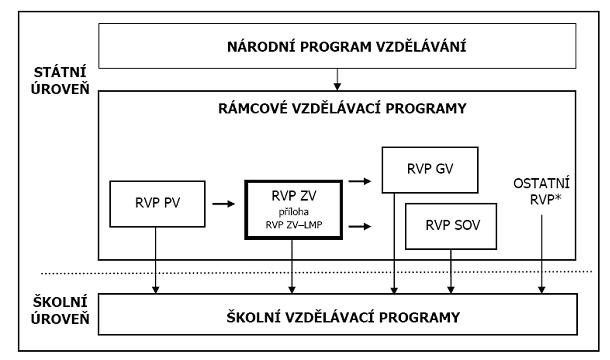
\includegraphics[width=0.8\linewidth]{fotky/rvpCR.jpg}
			\caption{
				\textbf{Rámcový vzdělávací program České republiky.}
				Schéma znázorňuje státní a~školní úroveň zpracovávání vzdělávacích programů.
			}
			\label{obr:rvpCR}
		\end{figure}

		%HACK
		\break \noindent
		Rámcový vzdělávací program pro předškolní vzdělávání je rozdělen do 12 kapitol, které jsou uvedeny v~originálním znění. \citep[s.~2]{RVP}
		\begin{enumerate}[1]
			\setlength\itemsep{-2mm}

			\item Vymezení Rámcového vzdělávacího programu pro předškolní vzdělávání v systému kurikulárních dokumentů
			\item Předškolní vzdělávání v systému vzdělávání a~jeho organizace
			\item Pojetí a~cíle předškolního vzdělávání
			\item Vzdělávací obsah RVP PV
			\item Vzdělávací oblasti
			\item Vzdělávací obsah ve školním vzdělávacím programu 
			\item Podmínky předškolního vzdělávání
			\item Vzdělávání dětí se speciálními vzdělávacími potřebami a~dětí mimořádně nadaných
			\item Autoevaluace mateřské školy a~hodnocení dětí
			\item Zásady pro zpracování školního vzdělávacího programu
			\item Kriteria souladu rámcového a~školního vzdělávacího programu
			\item Povinnost předškolního pedagoga
		\end{enumerate}

		Pro účely této práce a~možnosti komparace s francouzským kurikulem je nutné se podrobněji zabývat jen některými částmi RVP PV. Jedná se o~bod 3 \emph{Pojetí a~cíle předškolního vzdělávání} a~bod 5 \emph{Vzdělávací oblasti}.
		Obsah RVP je udáván pouze obecně a~rámcově, slouží jako prostředek k naplňování
		vzdělávacích záměrů a~dosahování vzdělávacích cílů. Vzdělávací obsah RVP PV je rozdělen do pěti oblastí:

		\begin{enumerate}[1]
			\setlength\itemsep{-2mm}
			\item Dítě a~jeho tělo
			\item Dítě a~jeho psychika
			\item Dítě a~ten druhý
			\item Dítě a~společnost
			\item Dítě a~svět
		\end{enumerate}

		Každá oblast obsahuje čtyři části. Těmito částmi jsou dílčí vzdělávací cíle (co pedagog u~dítěte podporuje), vzdělávací nabídka (co pedagog dítěti nabízí), očekávané výstupy (co dítě na konci předškolního období zpravidla dokáže) a~rizika (co ohrožuje úspěch vzdělávacích záměrů pedagoga).

		Mají-li se srovnávat vzdělávací oblasti a~jejich cíle u~obou dokumentů, je potřeba v~další kapitole uvést obsahy vzdělávácích oblastí rámcového vzdělávacího programu pro předškolní vzdělávání České republiky. Z~nich je níže uveden stručný výpis nejdůležitějších bodů. 

			\subsection{Dítě a~jeho tělo}
				\textit{\uv{Záměrem vzdělávacího úsilí pedagoga v oblasti biologické je stimulovat a~podporovat růst a neurosvalový vývoj dítěte, podporovat jeho fyzickou pohodu, zlepšovat jeho tělesnou zdatnost i~pohybovou a~zdravotní kulturu, podporovat rozvoj jeho pohybových a manipulačních dovedností, učit je sebeobslužným dovednostem a~vést je k zdravým životním návykům a~postojům.}} \citep[s.~16]{RVP}

				\paragraph{Dílčí vzdělávací cíle} 

				\begin{itemize}
				\setlength\itemsep{-2mm}
					\item[-]rozvoj jemné a~hrubé motoriky
					\item[-]uvědomění si a~ovládání vlastního těla
					\item[-]rozvoj všech smyslů
					\item[-]rozvoj psychické a~fyzické zdatnosti
					\item[-]základní poznatky o~zdraví a~zdravém životním stylu
				\end{itemize}

				\paragraph{Vzdělávací nabídka}

				\begin{itemize}
				\setlength\itemsep{-2mm}
					\item[-]lokomoční a~manipulační hry
					\item[-]smyslové a~psychomotorické hry
					\item[-]konstruktivní a~grafické hry
					\item[-]hudební a~hudebně pohybové hry
					\item[-]sebeosblužné činnosti
					\item[-]relaxační a~odpočinkové činnosti
					\item[-]prevence úrazů, nemoci, závislostí
				\end{itemize}

				\paragraph{Očekávané výstupy}

				\begin{itemize}
				\setlength\itemsep{-2mm}
					\item[-]správné držení těla
					\item[-]zvládnutí základních pohybových dovedností a~prostorové orientace
					\item[-]koordinace lokomoce, koordinace ruky a~oka a~jemné motoriky
					\item[-]napodobování pohybů podle vzoru
					\item[-]ovládání dechového svalstva
					\item[-]vnímat a~rozlišovat všemi smysly
					\item[-]zvládnutá sebeobsluha a~hygienické návyky
					\item[-]pojmenovat části těla a~jejich funkce
					\item[-]povědomí o~ochraně osobního zdraví a~kde hledat pomoc
				\end{itemize}

			\subsection{Dítě a~jeho psychika}
				\textit{\uv{Záměrem vzdělávacího úsilí pedagoga v oblasti psychologické je podporovat duševní pohodu, psychickou zdatnost a~odolnost dítěte, rozvoj jeho intelektu, řeči a~jazyka, poznávacích procesů a~funkcí, jeho citů i~vůle, stejně tak i~jeho sebepojetí a~sebenahlížení, jeho kreativity a~sebevyjádření, stimulovat jeho osvojování a~rozvoj jeho vzdělávacích dovedností a~povzbuzovat je v dalším rozvoji a~učení.
				Tato oblast zahrnuje tři „podoblasti“: Jazyk a~řeč; Poznávací schopnosti a~funkce, představivost a~fantazie, myšlenkové operace; Sebepojetí, city a~vůle.}} \citep[s.~18]{RVP}
				\paragraph{I~Jazyk a~řeč}
				 
					\subparagraph{Dílčí vzdělávací cíle}

					\begin{itemize}
					\setlength\itemsep{-2mm}
						\item[-]rozvoj řečových schopností a~jazykových dovedností  (receptivních i~produktivních)
						\item[-]rozvoj komunikativních dovedností
						\item[-]osvojení si dovedností předcházejících čtení a~psaní
					\end{itemize}
					
					\subparagraph{Vzdělávací nabídka}

					\begin{itemize}
					\setlength\itemsep{-2mm}
						\item[-]artikulační, řečové, sluchové a~rytmické hry
						\item[-]individuální a~skupinová  konverzace
						\item[-]vyprávění, komentování zážitků, vyřizování vzkazů
						\item[-]poslech pohádek, filmové a~divadelní příběhy
						\item[-]vyprávění, přednes, recitace, zpěv
						\item[-]grafické napodobování symbolů
						\item[-]poznávání a~rozlišování zvuku a~gest
						\item[-]seznámení se se sdělovacími prostředky
					\end{itemize}

					\subparagraph{Očekávané výstupy}

					\begin{itemize}
					\setlength\itemsep{-2mm}
						\item[-]správně vyslovovat, ovládat dech, tempo a~intonaci řeči
						\item[-]vyjadřovat myšlenky, nápady, pocity
						\item[-]vést rozhovor, domluvit se slovy i~gesty
						\item[-]porozumět slyšenému, formulovat otázky, odpovídat, slovně reagovat
						\item[-]umět krátké texty zpaměti, sledovat a~vyprávět příběh, popsat situaci, chápat slovní humor
						\item[-]sluchově rozlišovat začáteční a~koncové slabiky a~hlásky ve slovech, utvořit jednoduchý rým
						\item[-]poznat některá písmena, číslice, své jméno
						\item[-]zájem o~knížky, hudbu, film
					\end{itemize}
				
				\paragraph{II Poznávací schopnosti a~funkce, představivost a~fantazie, myšlenkové operace}
				\textcolor{white}{ } 

					\subparagraph{Dílčí vzdělávací cíle}

					\begin{itemize}
					\setlength\itemsep{-2mm}
						\item[-]rozvoj smyslového vnímání
						\item[-]rozvoj paměti, pozornosti, představivosti a~fantazie
						\item[-]rozvoj tvořivosti
						\item[-]posilování poznávacích citů
						\item[-]rozvoj zájmu o~učení
						\item[-]osvojení si elementárních poznatků o~znakových systémech
						\item[-]základ práce s~informacemi
					\end{itemize}
					
					\subparagraph{Vzdělávací nabídka}

					\begin{itemize}
					\setlength\itemsep{-2mm}
						\item[-]pozorování přírodních, kulturních a~technických objektů a~jevů
						\item[-]pojmenování jejich vlastností a~charakteristických znaků
						\item[-]motivovaná manipulace s~předměty
						\item[-]konkrétní manipulace s~materiálem
						\item[-]smyslové hry
						\item[-]hry na rozvoj postřehu, vnímání, zrakové a~sluchové paměti, pozornosti a~různých druhů paměti
						\item[-]námětové hry, hry podporující tvořivost, představivost a~fantazii
						\item[-]řešení myšlenkových i~praktických problémů a~hledaní řešení
						\item[-]činnosti k~seznámení s~matematickými pojmy a~jejich symbolikou
						\item[-]činnosti zasvěcující do časových pojmů
					\end{itemize}

					\subparagraph{Očekávané výstupy}

					\begin{itemize}
					\setlength\itemsep{-2mm}
						\item[-]vědomě využívat všech smyslů
						\item[-]záměrně pozorovat, všímat si, soustředit se a~udržet pozornost
						\item[-]poznat a~pojmenovat většinu toho, co ho obklopuje
						\item[-]přemýšlet a~vést jednoduché úvahy
						\item[-]naučit se nazpaměť krátké texty
						\item[-]postupovat a~učit se podle instrukcí, využívat zkušenost k~učení
						\item[-]chápat základní číselné a~matematické pojmy, souvislosti a~prakticky je používat
						\item[-]chápat prostorové pojmy, elementární časové pojmy
						\item[-]řešit problémy, myslet kreativně, nalézat nová řešení
						\item[-]vyjadřovat představivost v~tvořivých činnostech
					\end{itemize}
									
				\paragraph{III Sebepojetí, city, vůle}
				
					\subparagraph{Dílčí vzdělávací cíle}

					\begin{itemize}
					\setlength\itemsep{-2mm}
						\item[-]poznávání sebe sama, rozvoj pozitivních citů k~sobě
						\item[-]získání relativní citové samostatnosti
						\item[-]rozvoj schopnosti sebeovládání
						\item[-]vytváření osobních vazeb
						\item[-]rozvoj schopností vyjádřit prožitky a~dojmy
						\item[-]rozvoj mravního i~estetického vnímání
						\item[-]získání schopnosti záměrně řídit svoje chování a~ovlivňovat vlastní situaci
					\end{itemize}

					\subparagraph{Vzdělávací nabídka}
					
					\begin{itemize}
					\setlength\itemsep{-2mm}
						\item[-]spontánní hra
						\item[-]činnosti vyvolávající spokojenost, veselí, pohodu
						\item[-]úkoly, v~nichž může být dítě úspěšné
						\item[-]činnosti vyžadující samostatné vystupování, obhajování vlastních názorů, rozhodování, sebeohodnocení
						\item[-]hry pro rozvoj vůle a~sebeovládání
						\item[-]cvičení organizačních dovedností
						\item[-]estetické a~tvůrčí aktivity, cvičení v~projevování citů, v~sebekontrole a~sebeovládání
						\item[-]výlety do okolí
						\item[-]činnosti k~poznávání různých lidských vlastností
						\item[-]dramatické činnosti, mimické vyjadřování
						\item[-]činnosti vedoucí k~vyjádření sebe sama a~k~odlišení od ostatních
					\end{itemize}
					
					\subparagraph{Očekávané výstupy}

					\begin{itemize}
					\setlength\itemsep{-2mm}
						\item[-]odloučit se na určitou dobu od rodičů, uvědomovat si svou samostatnost
						\item[-]zaujímat vlastní názory, rozhodovat o~svých činnostech
						\item[-]vyjádřit souhlas i~nesouhlas, uvědomovat si své možnosti i~limity
						\item[-]přijímat pozitivní ocenění i~případný neúspěch a~vyrovnat se s~ním
						\item[-]vyvinout volní úsilí, soustředit se na činnost a~dokončit ji
						\item[-]zorganizovat hru a~respektovat pravidla
						\item[-]rozlišovat citové projevy v~různých prostředích, prožívat a~projevovat, co cítí
						\item[-]snažit se ovládat afektivní chování
						\item[-]být citlivý k~živým bytostem, přírodě i~věcem
						\item[-]těšit se z~příjemných zážitků
						\item[-]zachytit a~vyjádřit své pocity
					\end{itemize}

			\subsection{Dítě a~ten druhý}
				\textit{\uv{Záměrem vzdělávacího úsilí pedagoga v interpersonální oblasti je podporovat utváření vztahů dítěte k jinému dítěti či dospělému, posilovat, kultivovat a~obohacovat jejich vzájemnou komunikaci a~zajišťovat pohodu těchto vztahů.}} \citep[s.~24]{RVP}

					\paragraph{Dílčí vzdělávací cíle}

					\begin{itemize}
					\setlength\itemsep{-2mm}
						\item[-]seznamování se s~pravidly chování k~druhému
						\item[-]osvojení si schopností a~dovedností pro navazování a~rozvíjení vztahů
						\item[-]posilování prosociálního chování
						\item[-]vytváření prosociálních postojů
						\item[-]rozvoj komunikativních a~kooperativních dovedností
						\item[-]ochrana osobního soukromí
					\end{itemize}
					
					\paragraph{Vzdělávací nabídka}

					\begin{itemize}
					\setlength\itemsep{-2mm}
						\item[-]běžné komunikační aktivity dítěte s~druhými
						\item[-]sociální hry, hraní rolí, dramatické činnosti
						\item[-]hudební a~hudebně pohybové hry
						\item[-]aktivity podporující uvědomování si vztahů mezi lidmi
						\item[-]činnosti na porozumění pravidlům vzájemného soužití
						\item[-]hry vedoucí k~ohleduplnosti k~druhému, ochotě rozdělit se, pomoci si, vyřešit spor
						\item[-]činnosti na poznávání sociálního prostředí (rodina, MŠ)
						\item[-]hry, kdy se dítě učí chránit soukromí a~bezpečí své i~druhých
						\item[-]četba, vyprávění a~poslech příběhu s~etickým obsahem a~ponaučením
					\end{itemize}
					
					\paragraph{Očekávané výstupy}

					\begin{itemize}
					\setlength\itemsep{-2mm}
						\item[-]navazovat kontakty s~dospělým, kterému je svěřeno do péče
						\item[-]komunikovat s~ním, respektovat ho, porozumět projevům emocí a~nálad
						\item[-]přirozeně komunikovat s~druhým dítětem, navazovat přátelství
						\item[-]uvědomovat si svá práva a~respektovat práva ostatních
						\item[-]uplatňovat své individuální potřeby a~přání s~ohledem na druhé
						\item[-]dodržovat pravidla vzájemného soužití v~různých prostředích i~pravidla her
						\item[-]respektovat potřeby jiného dítěte, dělit se s~ním o~věci
						\item[-]vycházet vstříc ostatním a~pomáhat jim
						\item[-]bránit se projevům násilí
						\item[-]chovat se obezřetně při setkáních s~neznámými dětmi a~dospělými
					\end{itemize}

			\subsection{Dítě a~společnost}
				\textit{\uv{Záměrem vzdělávacího úsilí pedagoga v oblasti sociálně-kulturní je uvést dítě do společenství ostatních lidí a~do pravidel soužití s ostatními, uvést je do světa materiálních i~duchovních hodnot, do světa kultury a~umění, pomoci dítěti osvojit si potřebné dovednosti, návyky i~postoje a~umožnit mu aktivně se podílet na utváření společenské pohody ve svém sociálním prostředí.}} \citep[s.~26]{RVP}

					\paragraph{Dílčí vzdělávací cíle}

					\begin{itemize}
					\setlength\itemsep{-2mm}
						\item[-]poznávání pravidel společenského soužití a~jejich spoluvytváření
						\item[-]porozumění základním projevům neverbální komunikace v~tomto prostředí
						\item[-]rozvoj schopnosti žít ve společenství ostatních lidí a~přijímat základní hodnoty v~tomto společenství uznávané
						\item[-]rozvoj základních kulturně společenských postojů
						\item[-]rozvoj schopnosti projevovat se autenticky a~autonomně
						\item[-]vytvoření povědomí o~morálních hodnotách
						\item[-]seznamování se světem lidí, kultury a~umění
						\item[-]vytváření povědomí o~jiných kulturách, rozvoj společenského i~estetického vkusu
					\end{itemize}

					\paragraph{Vzdělávací nabídka}

					\begin{itemize}
					\setlength\itemsep{-2mm}
						\item[-]setkávání s~pozitivními vzory vztahů a~chování
						\item[-]aktivity pro adaptaci dítěte v~MŠ
						\item[-]společenské hry a~skupinové aktivity umožňující dětem se spolupodílet na jejich průběhu
						\item[-]přípravy a~realizace společenských zábav a~slavností
						\item[-]tvůrčí a~receptivní činnosti slovesné, literární, dramatické, výtvarné apod.
						\item[-]návštěvy kulturních a~uměleckých míst
						\item[-]hry na poznávání různých společenských rolí
						\item[-]aktivity přibližující pravidla vzájemného styku a~mravní hodnoty
						\item[-]hry a~praktické činnosti uvádějící dítě do světa lidí, jejich občanského života a~práce
						\item[-]aktivity přibližující svět kultury a~umění a~umožňující poznat rozmanitost kultur
					\end{itemize}
					
					\paragraph{Očekávané výstupy}

					\begin{itemize}
					\setlength\itemsep{-2mm}
						\item[-]uplatňovat návyky společenského chování ve styku s~dospělými i~dětmi
						\item[-]pochopit, že každý má ve společenství svou roli a~podle ní se chovat
						\item[-]chovat se dle vlastních pohnutek, ale s~ohledem na druhé
						\item[-]začlenit se do třídy a~respektovat rozdílné vlastnosti vrstevníků
						\item[-]porozumět běžným neverbálním projevům citových prožitků a~nálad druhých
						\item[-]adaptovat se ve škole a~zvládat požadavky prostředí
						\item[-]vyjednávat s~ostatními a~domluvit se na společném řešení
						\item[-]utvořit si základní dětskou představu o~pravidlech chování a~společenských normách a~chovat se dle toho
						\item[-]jednat spravedlivě, hrát fér, dodržovat pravidla her 
						\item[-]odmítat společensky nežádoucí chování a~chránit se před ním
						\item[-]vnímat umělecké podněty a~hodnotit svoje zážitky
						\item[-]vyjadřovat se pomocí výtvarných technik a~prostřednictvím hudeních a~hudebně pohybových činností
					\end{itemize}

			\subsection{Dítě a~svět}
				\textit{\uv{Záměrem vzdělávacího úsilí pedagoga v environmentální oblasti je založit u~dítěte elementární povědomí o~okolním světě a~jeho dění, o~vlivu člověka na životní prostředí – počínaje nejbližším okolím a~konče globálními problémy celosvětového dosahu – a~vytvořit elementární základy pro otevřený a~odpovědný postoj dítěte (člověka) k životnímu prostředí.}} \citep[s.~29]{RVP}

				\paragraph{Dílčí vzdělávací cíle}

				\begin{itemize}
				\setlength\itemsep{-2mm}
					\item[-]seznamování se a~vytváření si pozitivního vztahu k~místu a~prostředí, ve kterém dítě žije
					\item[-]poznávání jiných kultur
					\item[-]vytváření povědomí o~širším přírodním, kulturním i~technickém prostředí
					\item[-]pochopení, že lidská činnost může prostředí chránit, ale i~ničit
					\item[-]osvojení si poznatků péče o~okolí a~spoluvytváření zdravého prostředí
					\item[-]rozvoj úcty k~životu ve všech jeho formách
					\item[-]rozvoj schopnosti přizpůsobovat se podmínkám prostředí
					\item[-]vytvoření povědomí o~vlastní sounáležitosti se světem
				\end{itemize}
				
				\paragraph{Vzdělávací nabídka}

				\begin{itemize}
				\setlength\itemsep{-2mm}
					\item[-]přirozené pozorování prostředí a~života v~něm
					\item[-]aktivity zaměřené na praktickou orientaci v~obci
					\item[-]poučení o~možných nebezpečných situacích a~způsobech, jak se chránit
					\item[-]aktivity na téma dopravy, cvičení bezpečného chování v~dopravních situacích
					\item[-]poznávání přírodního okolí, sledování rozmanitostí a~změn v~přírodě
					\item[-]využívání encyklopedií a~obrazového materiálu
					\item[-]kognitivní činnosti, praktické činnosti k~seznámení s~materiály
					\item[-]pozorování životních podmínek a~životního prostředí a~okolní krajinu
				\end{itemize}
				
				\paragraph{Očekávané výstupy}

				\begin{itemize}
				\setlength\itemsep{-2mm}
					\item[-]bezpečně se orientovat ve známém prostředí
					\item[-]zvládat běžné činnosti a~požadavky na dítě kladené
					\item[-]chovat se přiměřeně a~bezpečně doma i~na veřejnosti
					\item[-]uvědomovat si nebezpečí a~jak se chránit
					\item[-]osvojit si elementární poznatky o~okolním prostředí
					\item[-]vnímat, že svět má svůj řád, že je rozmanitý a~pestrý
					\item[-]všímat si změn v~okolí a~porozumět, že změny jsou přirozené a~samozřejmé
					\item[-]mít povědomí o~významu životního prostředí
					\item[-]pomáhat pečovat o~okolní prostředí a~rozlišovat aktivity, které mohou zdraví okolního prostředí podporovat či poškozovat
				\end{itemize}

 			\subsection{Shrnutí cílů a~pojetí předškolního vzdělávání a~role pedagoga}

				V~českém dokumentu se pojetím a~cíli předškolní vzdělávání věnuje samostatná kapitola \uv{Pojetí a~cíle předškolního vzdělávání}. Níže shrnuto několik důležitých témat včetně vymezení role pedagoga a~doporučení pro jeho práci, volbu vhodných metod vzdělávání a~postupů. Výstupy vzdělávácích cílů předškolního vzdělávání jsou formulovány jako klíčové kompetence.			

				Mezi hlavní principy RVP PV patří akceptování přirozených vývojových specifik dětí předškolního věku, vzdělávání dítěte v rozsahu jeho individuálních možností a~potřeb, vytváření základů a~osvojení si klíčových kompetencí (viz níže) dosažitelných v etapě předškolního vzdělávání a~získávání předpokladů pro celoživotní vzdělávání.
				Předškolní vzdělávání má dítěti usnadňovat jeho další životní i~vzdělávací cestu, rozvíjet jeho osobnost, tělesný rozvoj a~zdraví, osobní spokojenost a~pohodu a~napomáhat mu v chápání okolního světa a~motivovat jej k dalšímu poznávání, stejně tak jako učit dítě žít ve společnosti ostatních a~přibližovat mu normy a~hodnoty uznávané touto společností.
				Vhodnými metodami vzdělávání je dle RVP PV prožitkové a~kooperativní učení hrou. Jde o činnosti, které jsou založeny na přímých zážitcích dítěte, které podporují dětskou zvídavost a~potřebu objevovat, podněcují jeho radost z učení a~jeho zájem poznávat nové věci a~získávat nové zkušenosti.
				RVP řadí situační učení a~spontánní sociální učení mezi významné procesy učení, které by měly být dostatečně zastoupeny. Střídat by se měly spontání a~řízené aktivity a~měly by být vzájemně provázané a~vyvážené. Pedagog by měl být průvodcem dítěte, probouzet v něm aktivní zájem a~chuť dívat se kolem sebe, naslouchat a~objevovat. Není zde jako ten, který „úkoluje“ a~kontroluje. Didaktický styl by měl být založen na principu vzdělávací nabídky, na individuální volbě dítěte a~jeho aktivní účasti.
				

				Důležitou složkou RVP PV jsou výstupy vzdělávacích cílů. Těmi jsou klíčové kompetence, neboli kompetence, které by děti měly ovládat na konci mateřské školy a~před vstupem do školy základní. Je zde uvedeno pět kompetencí. Ke každé z nich je uveden opět stručný výtah:

				\paragraph{Kompetence k učení}
				\begin{itemize}
				\setlength\itemsep{-2mm}
				\item[-] elementární poznatky o~světě lidí, kultuře, přírodě a~technice, která dítě obklopuje
				\item[-] orientace se v řádu dění
				\item[-] klást otázky a~hledat na ně odpovědi
				\item[-] aktivně si všímat a~chtít porozumět jevům, které kolem sebe vidí
				\item[-] soustředěně pozorovat, objevovat, experimentovat a získanou zkušenost dále uplatňovat
				\item[-] učení probíhá spontánně, vědomě, s~chutí
				\item[-] schopnost soustředit se na činnost a~dokončit práci
				\item[-] postupovat podle instrukcí, odhadovat své síly 
				\end{itemize}
				

				\paragraph{Kompetence k řešení problémů}
				\begin{itemize}
				\setlength\itemsep{-2mm}
				\item[-] všímat si dění i~problémů okolo sebe
				\item[-] známé situace řešit samostatně, náročnější s oporou a~pomocí dospělého
				\item[-] řešit problémy  na základě bezprostřední zkušenosti, cestou pokusu a~omylu experimentovat, vymýšlet nová řešení, hledat varianty
				\item[-] využívat dosavadních zkušeností, fantazii a~představivost 
				\item[-] užívat logických, matematických a~empirických postupů 
				\item[-] dovednost volit mezi řešením vedoucím k cíli a~řešením nefunkčním
				\item[-] nebát se chybovat
				\end{itemize}
				

				\paragraph{Kompetence komunikativní}
				\begin{itemize}
				\setlength\itemsep{-2mm}
				\item[-] v běžných situacích komunikovat bez zábran a~ostychu s dětmi i~s dospělými
				\item[-] ovládat řeč, samostatně vyjadřovat své myšlenky ve vhodně formulovaných větách
				\item[-] dokázat sdělit své prožitky a~pocity a~to všemi prostředky (i~výtvarnými, hudebními, dramatickými) 
				\item[-] ovládat dovednosti předcházející čtení a~psaní 
				\item[-] mít povědomí o~existenci jiných jazyků
				\item[-] průběžně rozšiřovat slovní zásobu a~aktivně ji používat
				\item[-] využívat informativní a~komunikační prostředky (telefon, knihy, počítač…)
				\end{itemize}

				\paragraph{Kompetence sociální a~personální}
				\begin{itemize}
				\setlength\itemsep{-2mm}
				\item[-] samostatně se rozhodovat o~svých činnostech
				\item[-] umět si vytvořit a~vyjádřit svůj názor
				\item[-] uvědomovat si, že odpovídá za své jednání, projevovat citlivost a~ohleduplnost k druhým, vnímat nespravedlnost a~ubližování
				\item[-] domlouvat se a~spolupracovat při společenských činnostech
				\item[-] uplatňovat pravidla společenského styku a~dodržovat dohodnutá pravidla 
				\item[-] respektovat druhé a~uzavírat kompromisy 
				\item[-] umět být tolerantní k odlišnostem druhých lidí
				\item[-] dokázat se bránit násilí a~ponižování
				\end{itemize}

				\paragraph{Kompetence činnostní a~občanské}
				\begin{itemize}
				\setlength\itemsep{-2mm}
				\item[-] dokázat rozpoznat svoje silné a~slabé stránky
				\item[-] učit se plánovat, organizovat a vyhodnocovat svoje činnosti a~hry
				\item[-] odhadovat rizika svých nápadů a~dokázat se přizpůsobovat okolnostem
				\item[-] chápat, že se může svobodně rozhodovat, ale i~že nese odpovědnost za svá rozhodnutí
				\item[-] zajímat se o~druhé a~o~to, co se děje kolem
				\item[-] mít smysl pro povinnost ve hře, práci i~učení
				\item[-] uvědomuje si svá práva i~práva druhých
				\item[-] uvědomovat si, že svým chováním ovlivňuje prostředí, ve kterém žije, a~dbát na osobní zdraví a~bezpečí své i~druhých
				\end{itemize}



\begin{landscape}
\begin{table}[t]
\center
\begin{tabular}{|c|c|c|l|}
\rowcolor{grey}
\hline			
				& \textbf{Francie}			& \textbf{Česká republika}	& \textbf{Rozdíly} 	\\
\hline
\hline
\rowcolor{grey!10}
Dokument	& státní, veřejně dostupný		& státní, veřejně dostupný 	& 			\\	\rowcolor{grey!50}
Rozsah		& 12 kapitol	 				& 11 kapitol	&						\\  \rowcolor{grey!10}
Předškolnímu vzdělání	& celý dokument			& 2 kapitoly	& FR: vzdělávání na půdě MŠ  zasahuje 	\\ \rowcolor{grey!10}
se věnuje				&						&				& do dvou vzdělávacích cyklů, proto  	\\ \rowcolor{grey!10}
				&								& 				& je prezentován v~jednom dokumentu  	\\ \rowcolor{grey!10}
				&								&				& společně s~ostatními cykly.    		\\ \rowcolor{grey!10}
				&								&				& ČR: preprimární vzdělávání odděleno 	\\ \rowcolor{grey!10}
				&								&				& od základního, věnuje se mu tedy  	\\ \rowcolor{grey!10}
				&								&				& samostatný dokument.					\\ 
\rowcolor{grey!50}
Kompetence		& na konci každé 				& hlavní výstupy  	&		\\	\rowcolor{grey!50}
				& vzdělávací oblasti 			& vzdělávacích cílů & 		\\
\rowcolor{grey!10}
Vzdělávací oblasti	& 6							& 5 					& FR: vzdělávací oblasti určují čeho 	\\	
\rowcolor{grey!10}
					& Osvojit si řeč			& Dítě a~jeho tělo		& má dítě dosáhnout.					\\
\rowcolor{grey!10}
					& Objevovat písmo 			& Dítě a~jeho psychika	& ČR: vzdělávací oblasti jsou sestave- \\
\rowcolor{grey!10}
					& Stát se žákem				& Dítě a~ten druhý	 	& né z~pozice dítěte k~obsahu. 			\\
\rowcolor{grey!10}
					& Jednat a~vyjadřovat se 	& Dítě a~společnost 	& 	 									\\
\rowcolor{grey!10}
					& vlastním tělem			& Dítě a~svět			& 	 									\\
\rowcolor{grey!10}
					& Objevovat svět			& 			 			& 	\\	
\rowcolor{grey!10}
					& Vnímat, cítit, 			& 						& 	\\
\rowcolor{grey!10}
					& představovat si, tvořit 	&						& 	\\		
\rowcolor{grey!50}
Dílčí vzdělávací cíle	& ANO					& ANO 					& 	\\	
\rowcolor{grey!10}
Vzdělávací nabídka	& Okrajově popsána	 		& Podrobně popsána	 	& Ve FR je dán větší prostor učitelům, 	\\
\rowcolor{grey!10}
					&							&						& jak budou práci koncipovat. 			\\
\rowcolor{grey!10}
					&							&						& V~ČR je tento prostor užší, nabídka 	\\
\rowcolor{grey!10}
					&							&						& je přesněji určena. 					\\
\rowcolor{grey!50}
Očekávané výstupy	& Formulované jako 				& Detailně popsány pro 		& 		\\ 
\rowcolor{grey!50}
					& kompetence na konci kapitoly 	& každou vzdělávací oblast 	& 		\\
\rowcolor{grey!10}
Rizika	 			& NE						& ANO	 						& 		\\
\hline
\end{tabular}
\caption{ \textbf{Srovnání kurikul Francie a~České republiky.}
}
\label{tab:srovnaniKurikul}
\end{table}
\end{landscape}

\section{Srovnání kurikul Francie a~České republiky}
\label{srovnanikurikulfrcr}

	Kurikulární dokumenty obou srovnávaných zemí, tedy Francie a~České republiky, mají stejné legislativní zázemí. Jsou to státní dokumenty zakotvené ve školském zákoně a~oba jsou volně dostupné široké veřejnosti jak pedagogické, tak nepedagogické. 

	Rozsah obou dokumentů je téměř shodný, avšak \textbf{český} Rámcový vzdělávací plán je zaměřen pouze na předškolní vzdělávání a~podrobně se věnuje všem oblastem, včetně rizik, které by mohly ohrozit úspěch vzdělávacích záměrů pedagoga, začleňování dětí se speciálními potřebami, podmínkám předškolního vzdělávání, autoevaluaci mateřských škol i~tvorbě školních vzdělávacích plánů. Jeho obsah je vyčerpávající a~zahrnuje všechny okolnosti, v~nichž se odehrává vývoj dítěte. 

	Oproti tomu je \textbf{francouzský} dokument rozsahem kratší a~věnuje se zvláště vzdělávacím oblastem a~cílům vzdělávání. Poslední třída mateřské školy je zároveň první třídou druhého vzdělávacího cyklu. Jde o~plynulý přechod na školu primární, tomu odpovídá i~obsah vzdělávání jak mateřské školy, tak prvních tříd školy základní. Cykly (viz kap. \ref{msvefr}) na sebe přirozeně navazují. Z~tohoto důvodu je program mateřských škol prezentován ve stejném dokumentu jako program primárního vzdělávání a~je mu věnována jeho poměrná část.

	Cíle v~\textbf{českém} RVP PV jsou podrobně rozpracovány na záměry a~výstupy. Formulovanými výstupy vzdělávacích cílů je 5 klíčových kompetencí, které jsou detailně popsány a~k jejichž naplňování by mělo směřovat veškeré vzdělávání v~mateřské škole. Ve \textbf{francouzském} Programu pro mateřské školy jsou kompetence zmíněné též, tzv. \uv{znalosti a~dovednosti, které by děti měly ovládat na konci MŠ}, ale jsou uvedeny na konci každé vzdělávací oblasti.

	Formulačně jsou vzdělávací oblasti obou dokumentů odlišné, ale při detailnějším čtení je zřejmé, že přestože jsou vzdělávací oblasti zařazené do jiných skupin, obsahují oba dokumenty tytéž oblasti, které je u~dětí potřeba systematicky rozvíjet. Nejmarkantnějšími rozdíly jsou ve francouzském programu v~obsahu oblastí \textit{Objevovat písmo} (Découvrir l´écrit) a~\textit{Stát se žákem} (Devenir élève).

	Ve \textbf{Francii} je kladen velký důraz na nácvik psaní. Na konci mateřské školy by děti měly ovládat velká tiskací písmena. Jak je v programu uvedeno, některým dětem se předkládá již písmo psací. Děti kopírují slova z~předloh, jako jsou dny v týdnu a~názvy měsíců v roce, a~učí se svému podpisu. V \textbf{České republice} se jedná spíše o~přípravu na psaní. Uvolňování svalů ruky, správné držení pera či tužky, nácvik grafomotoriky. Děti si uvědomují tvary, učí se uvolňovat zápěstí, ale neučí se psát konkrétní písmena a~nekopírují, s~výjimkou vlastního křestního jména. Písmena píší, jen když to vychází z jejich vlastního zájmu. 

	Název druhé zmíněné oblasti ve francouzském kurikulu \textit{Stát se žákem} evokuje přípravu na základní školu a~status žáka v~plném smyslu slova. Její obsah je společný s českými oblastmi \textit{Dítě a~ten druhý} a~\textit{Dítě a~společnost}, přestože z~pouhého názvu kapitol to není na první pohled patrné. Shoda kurikul obou zemí je ve formálním obsahu, ovšem v~pojetí hlavních vzdělávacích cílů se obě země diametrálně liší.

	Ve Francii si mateřská škola dává za úkol dostatečně dětem vštípit dovednosti a znalosti, které povedou k~úspěšnému zvládnutí základní školy. Formuje žáky a~uvádí je do světa psaného jazyka a~tím pádem i~do světa čtení. Během pozorování byl ve Francii znatelný rozdíl v~přístupu učitelů k~dětem, kterému je krátce věnována pozornost v~závěru kapitoly~\ref{srovnani}. Učitel rozdával \uv{úkoly}, děti \uv{pracovaly} (též viz kapitola ~\ref{dilny}). Autorka na základě kurikula a~vzdělávacích cílů vyvozuje, že na dítě je ve Francii pohlíženo jako na \uv{žáka}, a~tak se k~němu také přistupuje. 

	Mezi cíle předškolního vzdělávání v~České republice patří rozvoj osobnosti dítěte, jeho samostatnosti, rozvoj učení a~poznávání a~osvojení si hodnot naší společnosti. Vzdělávací oblasti jsou vzájemně provázány a~respektují přirozenost dítěte a~jeho postupné začleňování do životního a~sociálního prostředí. 

	Autorka se domnívá, že oproti Francii je v~českém předškolním vzdělávání více respektováno a~podporováno období dětství s~jeho vývojovými potřebami a~specifiky. Proto usuzuje, že v~České republice je na dítě pohlíženo jako na \uv{dítě}.
